\newpage
\section{Experimentos}

	En el presente capítulo se abordan las diferentes etapas que engloban a los experimentos de esta tesis. En las primeras 2 secciones se describen tanto las métricas y protocolos de evaluación utilizados en el dataset como así también los conjuntos de entrenamiento que se utilizan en los experimentos. Posteriormente, se detallan los parámetros que se utilizan en los diferentes experimentos y los resultados obtenidos de los mismos. Por último, se brinda un análisis de los resultados con el fin de evaluar la eficiencia del clasificador en las diferentes pruebas.

	\subsection{Métricas y Protocolo de Evaluación}

\FL{Explicar cómo se divide el dataset en train y test y qué métricas se calculan sobre el test (accuracy por ejemplo).}
	
	
	\subsection{Baselines}
\label{subsection:baseline}

	En esta sección se detallan los experimentos y los resultados obtenidos de realizar una reimplementación del trabajo de Wang et. al. en \cite{wang}. El objetivo es definir el baseline para el resto de los experimentos con imágenes reales y sintéticas. Así también, se definen los parámetros comunes a todos los experimentos como la configuración de HOG, $\alpha$ (parámetro de inicialización de las tablas), entre otros.
	
	Posteriormente se van a mostrar y explicar los resultados de los experimentos con imágenes reales. Se detalla el impacto de los diferentes esquemas de binarización con el fin de seleccionar el más adecuado para el resto de los experimentos.
	
	
\subsubsection{Reimplementación de Wang et. al.}

	En este experimento se utilizan, para el entrenamiento del clasificador, solamente imágenes de caracteres segmentados de escenas naturales e imágenes sintéticas (ver \ref{subsection:evaluacion}) siguiendo lo detallado por Wang et. al. en \cite{wang}. La evaluación del clasificador se realiza sobre un conjunto de prueba proporcionado por el dataset \textit{Chars74k-15} y se mantiene fijo durante todos los experimentos del presente trabajo.
	
	De la implementación de los autores, se pudieron obtener los siguientes parámetros para los experimentos:
	\begin{itemize}
		\item \textbf{Cantidad de grupos} ($M$): $256$.
		\item \textbf{Bits por grupo} (\textit{bpg}): $6$.
	\end{itemize}
	
	Estos dos valores generan vectores de características de longitud 1536.
	
	Para la función HOG,	 se utilizan dos parámetros, la cantidad de \textit{orientaciones} y la cantidad de \textit{celdas por bloque}. En los experimentos realizados, se prueban los siguientes conjuntos de valores:
	
	\begin{itemize}
		\item Orientaciones: $\textit{o} \in \{8, 9\}$
		\item Celdas por bloque: $\textit{cpb} \in \{4, 9\}$
	\end{itemize}
	
	En cuanto al método para binarizar los descriptores HOG, luego de haber leído la implementación provista por los autores, se establece como método la generación de variables aleatorias uniformes. Este enfoque, resultó ser el más adecuado debido a que es el que más se asemeja a lo que hicieron los autores en \cite{wang}	.
	
	Finalmente, el valor $\alpha$ para la inicialización de las tablas es un parámetro que no está especificado pero es necesario para poder entrenar el clasificador. En este experimento se probaron los siguientes valores de $\alpha$ con el fin de establecer el mejor valor.
	
	\begin{itemize}
		\item $\alpha \in \{0,01; 0,1; 1\}$.
	\end{itemize}
	
	Teniendo en cuenta estos parámetros, se obtuvieron los resultados que se pueden apreciar en el cuadro \ref{table: Baseline-Table}. En la misma, expresamos como ``NATIVE+FERNS'' a los resultados obtenidos al haber entrenado y evaluado el clasificador Random Ferns con imágenes reales. De la misma manera, ``SYNTH+FERNS'' se  refiere a los experimentos donde se usaron $1000$ imágenes sintéticas durante el entrenamiento.

	\begin{table}
		\centering
	    \begin{tabular}{ | l | l | l | p{5cm} |}
    			\hline
    				\textbf{Implementación} & \textbf{Score} \\ \hline
    				Wang NATIVE+FERNS & 54\% \\ \hline
    				Impl. propia NATIVE+FERNS & 50\% \\ \hline
    				Wang SYNTH+FERNS & 47\% \\ \hline
    				Impl. propia SYNTH+FERNS & 43\% \\

    			\hline
    		\end{tabular}
    		\caption[Resultados reales y sintéticas para baseline]{Resultados obtenidos en la reimplementación del trabajo de Wang et al.}
    		\label{table: Baseline-Table}
	\end{table}

	Como se puede ver en base a los resultados expuestos en el cuadro \ref{table: Baseline-Table}, hay diferencias significativas entre los resultados de ambas implementaciones que se deben a varios factores. Existen ciertos parámetros que no están especificados en el trabajo de Wang et al. y que se detallan a continuación:
	
	\begin{itemize}
		\item \textbf{Método de binarización}: El hecho de que en la reimplementación se utilizó un lenguaje diferente (Python), genera ciertos problemas. El uso de funciones que generan valores numéricos aleatorios depende mucho de la implementación de dichas funciones. Estas pueden variar entre los lenguajes por lo cual los resultados obtenidos son diferentes. La binarización hace uso de valores aleatorios con lo que se generan estas diferencias.
		\item \textbf{$\alpha$}: es el parámetro para la inicialización de las tablas que influye en la performance.
		\item \textbf{Implementación de HOG}: la implementación de HOG que usan los autores es la desarrollada por Piotr Dollár \cite{PiotrD} la cual es una variación del método original propuesto por Dalal \& Triggs en \cite{DT05}. En la reimplementación se utiliza la función HOG extraída de la librería de python scikit-images, que también está basada en \cite{DT05} pero difiere de la usada por los autores. Una de las diferencias entre ambas funciones está en que la desarrollada por Piotr Dollar acepta imágenes a color y la que se usa en este trabajo sólo acepta imágenes en escala de grises. Otra diferencia entre estas implementaciones está en la longitud del vector resultante. Usando los mismos parámetros en ambas funciones, la desarrollada por Piotr Dollar devuelve vectores con una longitud $4$ veces mayor a los devueltos por la función HOG usada en el presente trabajo. Esto se debe a que usa un esquema diferente de normalización.
	\end{itemize}
	
	Ante esta situación se decide por establecer como baselines los resultados obtenidos por la configuración más cercana a la usada en \cite{wang}. Teniendo en cuenta los parámetros conocidos, se establece además las siguiente configuración:
	
	\begin{itemize}
		\item \textbf{HOG}: se consideran $8$ orientaciones y $9$ celdas por bloque como los parámetros que mejores resultados produjeron.
		\item \textbf{$\alpha$}: se establece en $0.01$ pues es el valor que más impacto positivo produjo en estos experimentos.
	\end{itemize}		
	
	El esquema de binarización utilizado en este experimento sirve solamente para establecer el baseline para el resto de los experimentos. En la siguiente subsección se evalúan, a través de experimentos con imágenes reales, nuevos métodos de binarización (explicados en \ref{subsubsection:binarizacion}) y se va a considerar como baseline el valor $0.50$. De la misma manera, en la sección de los experimentos con imágenes sintéticas, el baseline pasará a ser $0.43$.
	
\subsubsection{Evaluación de Esquemas de Binarización}
\label{subsubsection: eval_esquemas}


	Esta subsección tiene como objetivo evaluar los 4 esquemas de binarización detallados en \ref{subsubsection:binarizacion}. Además, como resultado de los experimentos, se establecerá cúal es tamaño óptimo para los grupos o \textit{ferns} y cúal es la mejor dimensión para los vectores de características. Para esto, se entrena y evalua al clasificador \textit{Random Ferns} con imágenes reales de la misma manera que en la subsección anterior.
	
	Inicialmente, se van a mostrar $4$ gráficos, que corresponden a los métodos utilizados en la binarización. Con esto se busca ver qué método devuelve los mejores resultados. Estas figuras, reflejan la diferencia en performance al considerar grupos de diferente dimensión $B/G \in \{ 1, 4, 8, 10\}$. Con esto se busca establecer, para cada caso, qué dimensión arroja los mejores resultados. Cabe aclarar que cada gráfico refleja la media de los resultados de 5 corridas del experimento junto con las barras de error a 1 desviación estándar. La Figura \ref{fig: Reales-Comparativa metodos} reúne los mejores resultados de clasificación de las primeras cuatro figuras para establecer una comparación más precisa. En la tabla \ref{table: reales-comparativa} se muestra un resumen de los mejores valores.

	 Dada la gran cantidad de parámetros que se manejan en estos experimentos, se va a dejar detallado en el análisis cuales son los mejores y se los va a usar para los siguientes experimentos.

			\begin{figure}[htbp!]
				\centering
				\centerline{
					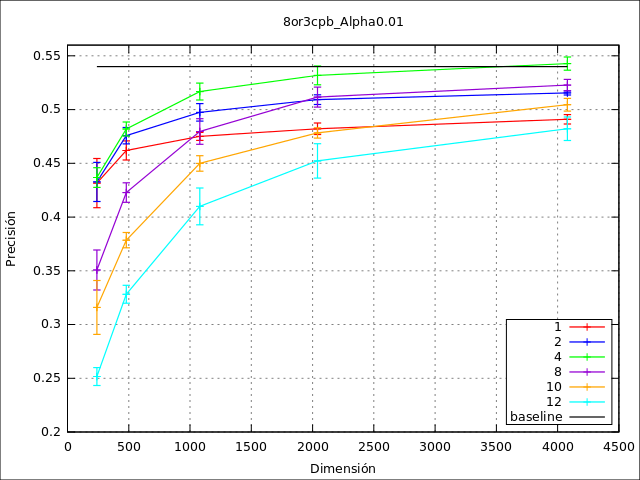
\includegraphics[scale=0.6]{img/resultados/reales/mean.png}
				}
				\caption[Resultados media]{Resultados usando la media}
				\label{fig: Reales-media}
			\end{figure}
			\begin{figure}[htbp!]
				\centering
				\centerline{
					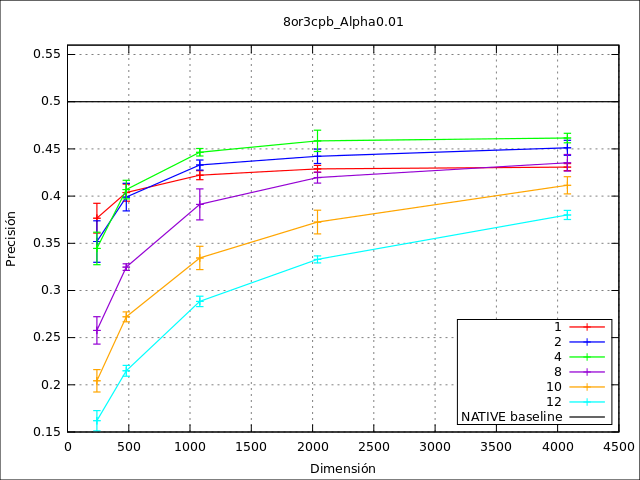
\includegraphics[scale=0.6]{img/resultados/reales/median.png}
				}
				\caption[Resultados mediana]{Resultados usando la mediana}
				\label{fig: Reales-mediana}
			\end{figure}
			\begin{figure}[htbp!]
				\centering
				\centerline{
					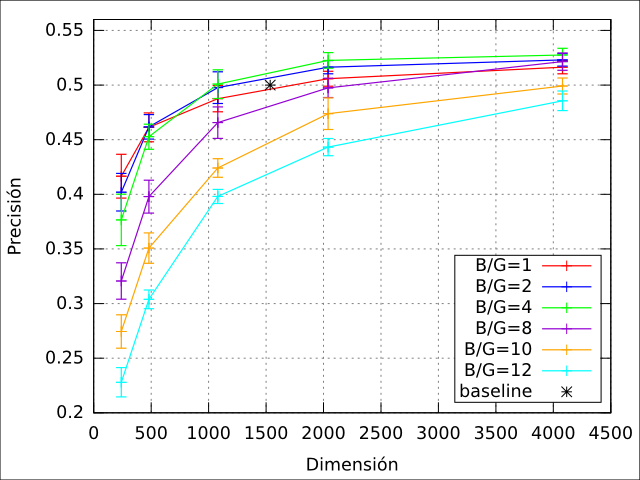
\includegraphics[scale=0.6]{img/resultados/reales/expon.png}
				}
				\caption[Resultados expon]{Resultados usando la distribución exponencial}
				\label{fig: Reales-expon}
			\end{figure}
			\begin{figure}[htbp!]
				\centering
				\centerline{
					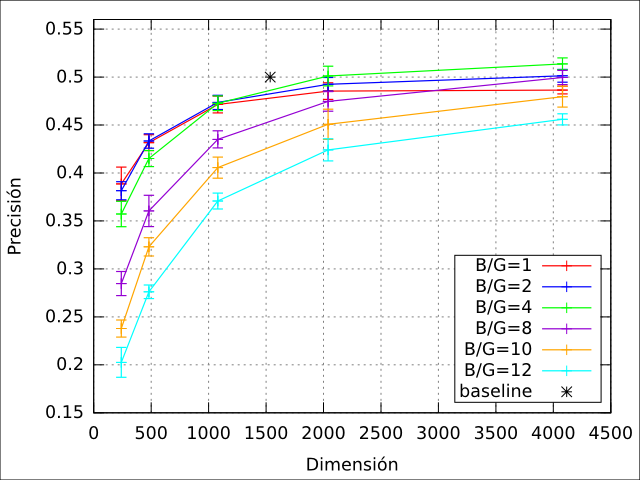
\includegraphics[scale=0.6]{img/resultados/reales/bootstrap.png}
				}
				\caption[Resultados bootstrap]{Resultados usando bootstrap}
				\label{fig: Reales-bootstrap}
			\end{figure}

	Teniendo en cuenta los resultados de los primeros $4$ gráficos, a simple vista se puede observar que los resultados obtenidos usando la media como método para binarizar los vectores son los mejores, llegando estos a un máximo cercano al $55\%$ de precisión. En el caso opuesto, el usar la mediana arrojó los peores resultados, ya que, en el mejor de los casos, se supera el $47\%$ a diferencia de bootstrap que llega a $51\%$ . El uso de la distribución exponencial en los casos donde la longitud de los grupos es baja ($1$ bit por grupo) no supera a la media en performance pero aumenta a medida que aumentamos este valor (casos $\{ 4, 8, 10\}$ bits por grupo). Los valores que podemos encontrar en \ref{fig: Reales-expon} se acercan a los del a media llegando a un máximo en la precisión de $53\%$. En cuanto al uso de bootstrap, se puede apreciar que los resultados se mantienen por debajo de los obtenidos con la distribución exponencial y la media con valores que rondan entre $45\%$ y $52\%$ (en el mejor de los casos).

	En cuanto a las dimensiones del vector binario evaluadas en el experimento $\{ 240, 480, 1080, 2040, 4080 \}$, es claro que a medida que aumentamos la longitud de los vectores aumenta la performance. Se puede ver que, cuando se usan vectores de longitud reducida (en este caso $240$), se marca una diferencia importante en la precisión entre los experimentos realizados con grupos de dimensionalidad baja $\{ 1, 4 \}$ y alta $\{8, 10\}$. Es decir, dejando fija la dimensión de los vectores en $240$, mientras más chico es el tamaño de los grupos mejor es el resultado (se puede observar en cualquiera de las figuras). En el otro extremo, si usamos grupos de $10$ bits la precisión disminuye considerablemente. La misma relación se mantiene a medida que aumentamos el tamaño de los vectores de características hasta cierto punto. Por ejemplo, en \ref{fig: Reales-media} es claro que a partir del uso de $1080$ como tamaño de vector en adelante, el uso de grupos de longitud mayor arroja mejores resultados. Lo mismo sucede en las otras figuras en diferentes puntos.

	En cuanto al uso del valor $4080$, se puede ver que no hay un aumento considerable en la performance que lo diferencie del uso de $2040$. Con esto en mente, es conveniente hacer uso de este último valor ya que usa vectores mucho más chicos incrementando la eficiencia en el cómputo.

	El enfoque del clasificador Ferns es semi-na\"{i}ve, es decir, a diferencia del clasificador Na\"{i}ve Bayes, se considera que hay cierta relación de dependencia o correlación entre las dimensiones del vector de características. Por lo tanto, tal y como se explica en \ref{subsection:ferns}, los vectores se dividen en grupos de dimensión \textit{S}. Esto con el objetivo de ir un paso más allá de la independencia propuesta en Na\"{i}ve Bayes donde cada dimensión es independiente y así poder capturar estas correlaciones. El problema con los vectores binarizados de dimensión reducida, es que almacenan menos información sobre los datos de la imagen a comparación de los vectores cuya longitud es mayor. En cada grupo, se capturan las correlaciones entre las dimensiones involucradas en estos, es decir, el nivel de dependencia o relación que existen entre las mismas. Es por eso que al aumentar la dimensionalidad de los vectores en el proceso de binarización, capturamos más estructuras de correlación de los datos. Basándonos en esto, y como se puede observar en los gráficos expuestos, los grupos de $4$ bits son los más adecuados en la clasificación en la mayoría de los casos.

			\begin{figure}[htbp]
				\centering
				\centerline{
					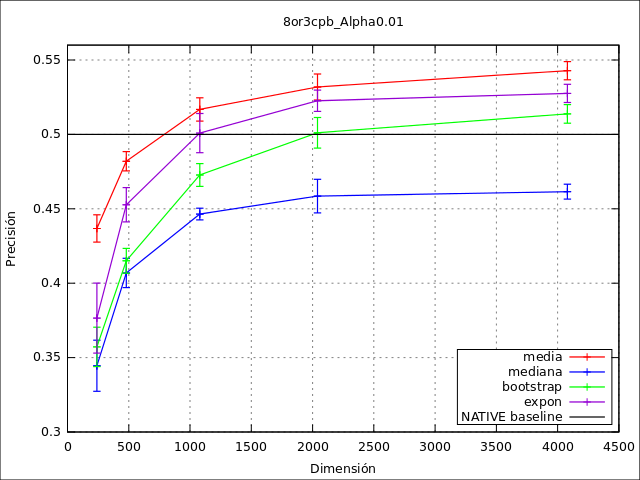
\includegraphics[scale=0.6]{img/resultados/reales/comparativa_metodos.png}
				}
				\caption[Reales comparativa]{El gráfico muestra las mejores curvas de los gráficos presentados con la mejor configuración}
				\label{fig: Reales-Comparativa metodos}
			\end{figure}

	Del análisis realizado surge que la mejor configuración está dada por: \textit{bits por grupo = $4$} y \textit{dimensión del vector = $2040$}. Se puede observar en \ref{fig: Reales-Comparativa metodos} las mejores curvas para cada método utilizando la mejor configuración (a excepción de la longitud del vector con el objetivo de ver la curva de crecimiento). Queda claro que la media se puede establecer como el mejor método para la binarización por lo que en los próximos experimentos se procederá a trabajar con este método de binarización. La diferencia en precisión entre usar vectores de longitud $2040$ y $4080$ no es notable en los $4$ casos por lo cual como dijimos anteriormente, el uso de $2040$ dimensiones permite obtener buenos resultados con un menor costo computacional. En todos los casos, salvo cuando se usa la mediana como método de binarización, se supera el baseline propuesto en diferentes puntos. La media logra una diferencia de $4\%$ con respecto al baseline pero usando vectores de dimensión $4080$, la misma diferencia baja a un $3\%$ si consideramos $2040$.

	La tabla \ref{table: reales-comparativa} muestra un resumen de los valores obtenidos con la mejor configuración para cada método.

	\begin{table}
		\centering
		\begin{tabular}{ | l | l | l | p{5cm} |}
    			\hline
    				\textbf{NATIVE + FERNS} & \textbf{Score} \\ \hline
    				Media & 53\% \\ \hline
    				Mediana & 46\%\\ \hline
    				Exponencial & 52\% \\ \hline
    				Bootstrap & 50\%\\
    			\hline
    		\end{tabular}
    		\caption[Resultados imágenes naturales]{Tabla comparativa entre los diferentes métodos propuestos para la binarización en la clasificación de caracteres en escenas naturales usando la mejor configuración de parámetros.}
    		\label{table: reales-comparativa}
    	\end{table}





	
	
	\subsection{Uso de imágenes sintéticas}

	En esta sección se busca ver el impacto producido por las imágenes sintéticas en la clasificación. Es decir, se buscar entrenar al clasificador con dos grupos de imágenes. El primer conjunto está conformado por imágenes sintéticas alteradas cuyo proceso de creación fue detallado en la sección \ref{subsection:impl_propia}. El segundo esta conformado por una combinación del primer grupo con el conjunto de imágenes reales usado en \ref{subsection:baseline}.
	
	El grupo de imágenes de fuentes sintéticas de computadora que se usa para crear los caracteres sintéticos fue extraído del dataset mencionado en \ref{subsection:evaluacion} y consiste en 1000 imágenes por clase. De este conjunto se crearon 6 variaciones diferentes, con el objetivo de observar el impacto que tiene la cantidad de caracteres sintéticos al momento de clasificar imágenes de caracteres naturales. La cantidad de muestras por clase (variaciones) en cada conjunto de entrenamiento es la siguiente:
	\begin{itemize}
		\item Muestras por clase : $ mpc \in \{ 50,100,250,500,1000,2000\}$
	\end{itemize}
	
	Estas variaciones son puestas a prueba en el primer experimento de la sección.
	
	El segundo conjunto de imágenes sintéticas se creó con la finalidad de observar el impacto en la clasificación de integrar, en diferentes proporciones, imágenes sintéticas y reales al conjunto de entrenamiento. Dada la escasa cantidad de imágenes naturales para el entrenamiento (15 en total por cada clase), se busca complementar esto integrando datos sintéticos. Por consiguiente, se decide crear 9 conjuntos de entrenamiento donde en cada uno se incorporan diferentes proporciones de imágenes sintéticas a las 15 reales existentes. La proporción de cada conjunto de entrenamiento es: 
	
	$$(15, x)~\textit{con}~ x \in \{0,3,8,15,30,75,150,300,750,1500 \}$$
	
	El primer elemento de la tupla $(15, x)$ corresponde a la cantidad de imágenes reales, cuyo valor es fijo. El segundo elemento de la tupla hace referencia a la proporción de caracteres sintéticos. Es fácil observar que a medida que aumentamos la proporción, la cantidad de caracteres naturales se va volviendo cada vez más despreciable. El hecho de no considerar imágenes sintéticas inicialmente $(15,0)$ tiene como finalidad el observar el cambio que se produce desde el inicio cuando no hay caracteres sintéticos en el entrenamiento.
	
	Este segundo grupo de imágenes es puesto a prueba en el último experimento de la sección.

	Los parámetros utilizados durante la creación de las imágenes sintéticas son, como se explicó en \ref{subsection:impl_propia}, escala, rotación, transvección, traslación, blur y ruido Gaussiano. Dado que hay un abanico bastante grande de valores para asignarles a estas transformaciones, se decidió por asignarle a cada una un rango de valores razonable. Dado que los autores en \cite{wang} no especifican el rango de valores para las transformaciones que utilizan, se procedió a establecer los siguientes intervalos para todas las transformaciones utilizadas:
	
	\begin{itemize}
		\item Transvección: $n \in [-0.20 ; 0.20]$
		\item Suavizado gaussiano (blur): $\sigma \in [0 ; 2]$
		\item Escala: $a=d \in [0.8; 1.25]$
		\item Rotación (en radianes): $\theta \in (-0.1; 0.1)$
		\item Ruido Gaussiano: $\sigma \in [1; 30]$
	\end{itemize}

\subsubsection{Primer Experimento: Conjunto de imágenes sintéticas}
\label{subsubsection:primer-experimento}

	En el primer experimento, se procederán a mostrar los resultados obtenidos de haber utilizado el primer conjunto de imágenes. Los gráficos van a representar la relación entre la cantidad de imágenes sintéticas por clase (dado por \textit{IPC} en las siguientes figuras) y la precisión de clasificación dada por los $4$ valores a evaluar que son las dimensiones de los grupos. Teniendo en cuenta los resultados anteriores con las imágenes reales, se decidió por trabajar con la mejor configuración encontrada salvo por el parámetro \textit{B/G}(\textit{bits por grupo}). Este último parámetro se mantuvo con el fin de seguir evaluándolo con estos nuevos experimentos.
	
	El baseline con el que se comparan los resultados es el obtenido en \ref{subsection: baseline} para las imágenes sintéticas cuyo valor es $0.43$.

			\begin{figure}[htbp]
				\centering
				\centerline{
					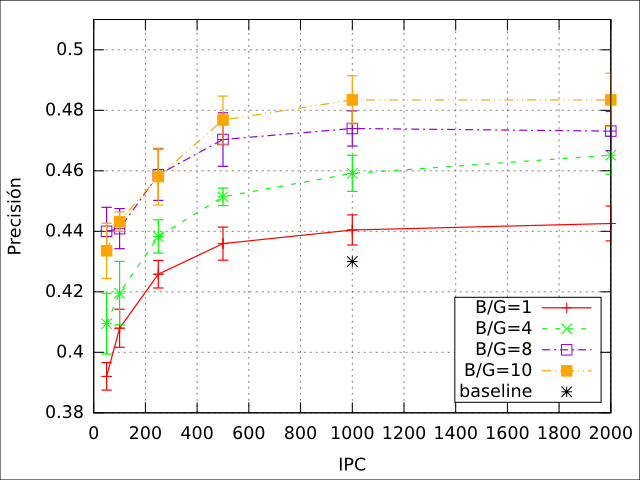
\includegraphics[scale=0.5]{img/resultados/sinteticas/mean_2040.png}
				}
				\caption[Sintéticas media 2040]{El gráfico muestra los resultados obtenidos de haber utilizado la mejor configuración analizada y haciendo uso de vectores binarizados de longitud $2040$.}
				\label{fig: Sinteticas-media-2040}
			\end{figure}

	En cuanto a los experimentos con imágenes sintéticas, basándonos en los resultados plasmados en la figura \ref{fig: Sinteticas-media-2040}, es interesante observar que a medida que agregamos más imágenes sintéticas por clase, aumenta la performance del clasificador en todos los casos. Inicialmente, el crecimiento es más pronunciado hasta llegar a un punto (a partir de las 1000 IPC) en donde el mismo no es tan notable y en algunos casos tiende a ``aplanarse''. En base a esto, no tiene sentido trabajar con más de $1000$ imágenes por clase, pues computacionalmente es más costoso y no se obtiene una precisión que justifique su uso. En el mejor de los casos, al usar grupos de $10$ bits, la diferencia en performance entre usar $1000$ ó $2000$ imágenes por clase es nula. El hecho de que se hayan necesitado $2000$ muestras por clase para alcanzar una performance cercana al $49\%$, también refleja que las imágenes sintéticas no aportan la misma cantidad de información que las reales.
	
	Una particularidad de este experimento con respecto a los anteriores (ver \ref{subsubsection: eval_esquemas}), es que los mejores resultados se obtienen cuando la cantidad de bit por grupo (dado por \textit{B/G} en \ref{fig: Sinteticas-media-2040}) es grande. Esta tendencia se ve en todos los niveles a medida que aumenta \textit{IPC}.

	Por último, en cuanto a la comparación con el baseline, los resultados en la mayoría de los casos son superiores incluso habiendo entrenado al clasificador con menos imágenes por clase ($\leq 1000$). Por lo tanto, se puede decir que la configuración elegida hace un mejor uso de los datos de entrenamiento.
	
\subsubsection{Segundo Experimento: Conjunto de imágenes mixto}
	
	En este último experimento, se van a mostrar los resultados correspondientes de haber entrenado al clasificador \textit{Random Ferns} con conjuntos de entrenamiento mixtos. Se procederá a mostrar la figura con la mejor configuración. También se mostrarán las matrices de confusión para este caso. Al igual que en \ref{subsubsection:primer-experimento}, se va a utilizar la mejor configuración obtenida en \ref{subsection:baseline} descartando también al parámetro $B/G$.

	El gráfico a continuación presenta el eje \textit{x} en escala logarítmica para poder apreciar mejor las variaciones que se dan al experimentar con valores cercanos entre sí.

			\begin{figure}[!htbp]
				\centering
				\centerline{
					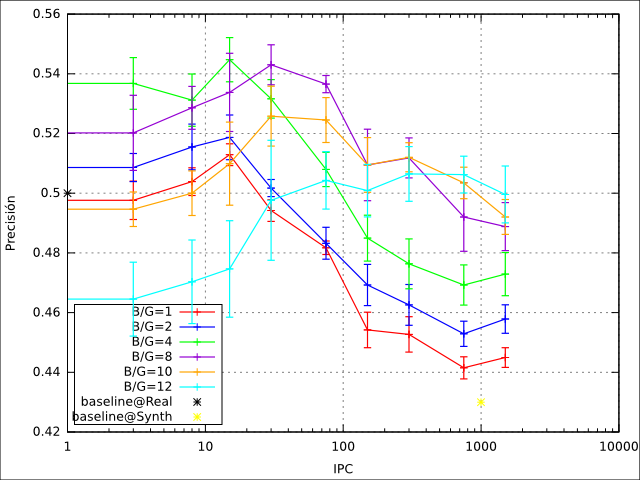
\includegraphics[scale=0.6]{img/resultados/mixtas/best_mean_2040.png}
				}
				\caption[Mixtas media mejor resultado]{El gráfico muestra la configuración que devolvió los mejores resultados.}
				\label{fig: Mixtas-media-mejor}
			\end{figure}

	De la figura \ref{fig: Mixtas-media-mejor} se puede desprender el siguiente análisis. El primero, y uno de los más importantes, hace referencia a la influencia en la clasificación de ir agregando de manera incremental imágenes sintéticas durante la etapa de entrenamiento. Se puede observar que a nivel general todos los experimentos llegaron a un punto donde su performance se desplomó al seguir agregando imágenes. Sin embargo, este cambio ocurrió en diferentes momentos dependiendo del caso. Por ejemplo, cuando trabajamos con grupos de dimensionalidad baja ($1$ y $4$ bits por grupo), la precisión del clasificador va en aumento hasta que se llega a un máximo correspondiente al haber entrenado al sistema con igual cantidad de imágenes reales y sintéticas. A partir de ese punto, el seguir incrementando la proporción de sintéticas sobre reales trajo efectos negativos en los resultados como se puede apreciar en el gráfico presentado. En los casos donde consideramos $10$ bits por grupo el rendimiento se desploma cuando consideramos más de 75 imágenes sintéticas. Cuando superamos esa proporción se puede ver que la performance decae. Todo esto se debe a que llegado cierto punto, el clasificador aprende las particularidades de los datos sintéticos. Es decir, a medida que la cantidad de imágenes sintéticas supera en gran proporción a la imágenes reales, la información almacenada sobre las primeras adquiere más relevancia en la clasificación haciendo que la performance disminuya.

	 La mejor curva en el gráfico la obtenemos cuando consideramos $4$ bits por grupo y entrenamos al clasificador con la misma cantidad de imágenes sintéticas que reales. Este resultado coincide respecto al análisis realizado para los experimentos con imágenes reales donde consideramos que el mejor parámetro era considerar grupos de $4$ bits. En la mayoría de los casos se dan buenos resultados cuando la cantidad de imágenes sintéticas sobre las reales es la misma ($1$ y $4$) o se duplica ($8$ y $10$).

	 Teniendo en cuenta los baselines presentados en la tabla \ref{table: Baseline-Table} y el hecho de que estos experimentos tienen una base inicial de imágenes reales, se puede observar que el baseline ``SYNTH'' es superado. En cuanto al baseline ``NATIVE'', a diferencia de los resultados obtenidos con las imágenes reales (que se pueden ver en el inicio de cada curva de la figura \ref{fig: Mixtas-media-mejor}), el incremento en la precisión del clasificador no es muy notorio; sin embargo, el hecho de poder incrementar la performance haciendo uso de imágenes sintéticas es un avance. Llama la atención que el usar la misma cantidad de imágenes reales y sintéticas no haya producido un incremento más marcado en la performance. Sin embargo, como pudimos ver en \ref{fig: Sinteticas-media-2040}, ni con 50 imágenes sintéticas por clase se podía alcanzar un valor similar al del baseline.

	Otro de los análisis realizado en el trabajo pasa por los errores de clasificación que se han observado. En las figuras \ref{fig: Mixtas-Matrix-media-mejor} y \ref{fig: MatrizIns-Mixtas-media-mejor}, se pueden ver dos matrices de confusión. La primer corresponde al mejor resultado obtenido en la figura \ref{fig: Mixtas-media-mejor} y la segunda es una versión de la primera donde no diferenciamos caracteres mayúsculas de minúsculas.

	En la región central, dada por la diagonal de la matriz, se encuentran las muestras que fueron bien clasificadas durante la evaluación del clasificador. Existen zonas dentro de la diagonal que corresponden a clases que obtuvieron una tasa de acierto inferior al $30\%$ (los cuadrados en escala de azul dentro de la imagen). En estas clases son más comunes los siguientes errores:

	\begin{itemize}
		\item No poder distinguir mayúsculas de minúsculas para los caracteres involucrados. En la figura \ref{fig: Error-CaseSensitive} se puede observar un ejemplo donde, incluso para las personas, es difícil notar la diferencia.
		\item Confundir un carácter por otro similar. La figura \ref{fig: Error-Apariencia} muestra varios ejemplos donde se pueden confundir caracteres.
	\end{itemize}

		\begin{figure}[htbp]
			\centering
			\subfloat[c minúscula\label{fig: Lower-case-c}]{
				\fbox{ 
\includegraphics[scale=1]{img/errores_clasif/CaseSensitiveError/lowerCase_c.png} }
			}
			\subfloat[C mayúscula\label{fig: Upper-case-C}]{
				\fbox{ 
\includegraphics[scale=1]{img/errores_clasif/CaseSensitiveError/upperCase_C.png} }
			}
			\subfloat[z minúscula\label{fig: Lower-case-z}]{
				\fbox{
\includegraphics[scale=1]{img/errores_clasif/CaseSensitiveError/lowerCase_z.png} }
			}
			\subfloat[Z mayúscula\label{fig: Upper-case-Z}]{
				\fbox{ 
\includegraphics[scale=1]{img/errores_clasif/CaseSensitiveError/upperCase_Z.png} }
			}
			\\
			\subfloat[x minúscula\label{fig: Lower-case-x}]{
				\fbox{ 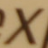
\includegraphics[scale=1]{img/errores_clasif/CaseSensitiveError/lowerCase_x.png} }
			}
			\subfloat[X mayúscula\label{fig: Upper-case-X}]{
				\fbox{ 
\includegraphics[scale=1]{img/errores_clasif/CaseSensitiveError/upperCase_X.png} }
			}
			\subfloat[v minúscula\label{fig: Lower-case-v}]{
				\fbox{ 
\includegraphics[scale=1]{img/errores_clasif/CaseSensitiveError/lowerCase_v.png} }
			}
			\subfloat[V mayúscula\label{fig: Upper-case-V}]{
				\fbox{ 
\includegraphics[scale=1]{img/errores_clasif/CaseSensitiveError/upperCase_V.png} }
			}
			\caption[Error entre mayúscula y minúscula]{Error de clasificación donde se confunde el carácter en mayúscula y en minúscula.}
			\label{fig: Error-CaseSensitive}
		\end{figure}

		\begin{figure}[htbp]
			\centering
			\subfloat[o minúscula\label{fig: Lower-case-o}]{
				\fbox{ 
\includegraphics[scale=1]{img/errores_clasif/ShapeError/lowerCase_o.png} }
			}
			\subfloat[O mayúscula\label{fig: Upper-case-O}]{
				\fbox{ 
\includegraphics[scale=1]{img/errores_clasif/ShapeError/upperCase_O.png} }
			}
			\subfloat[número 0\label{fig: Number-0}]{
				\fbox{
\includegraphics[scale=1]{img/errores_clasif/ShapeError/number_0.png} }
			}
			\\
			\subfloat[I mayúscula\label{fig: Upper-case-I}]{
				\fbox{ 
\includegraphics[scale=1]{img/errores_clasif/ShapeError/upperCase_I.png} }
			}
			\subfloat[l minúscula\label{fig: Lower-case-l}]{
				\fbox{ 
\includegraphics[scale=1]{img/errores_clasif/ShapeError/lowerCase_l.png} }
			}
			\subfloat[número 1\label{fig: Number-1}]{
				\fbox{ 
\includegraphics[scale=1]{img/errores_clasif/ShapeError/number_1.png} }
			}
			\caption[Error de apariencia]{Error de apariencia entre caracteres.}
			\label{fig: Error-Apariencia}
		\end{figure}


	El no poder distinguir mayúsculas de minúsculas se ve reflejado en la matriz \ref{fig: MatrizIns-Mixtas-media-mejor} en dos regiones. Dichas regiones corresponden a dos submatrices, la primera ubicada en la esquina inferior izquierda y la segunda en la esquina superior derecha. Ambas submatrices, no involucran los caracteres numéricos y se puede ver en la diagonal de cada una, la cantidad de imágenes de cada clase donde se confundió la versión mayúscula y minúscula. Es muy difícil, incluso para las personas, clasificar imágenes de caracteres recortados donde no hay una clara distinción entre la versión mayúscula y minúscula.

	Los errores de ``apariencia'' como los expuesto en la figura \ref{fig: Error-Apariencia} están distribuidos por toda la matriz, habiendo casos donde la similitud es evidente y en otros casos más raros donde no existe directamente. Este último caso, donde no existe similitud, puede solventarse si se entrenase al clasificador con más imágenes.

	La matriz \ref{fig: MatrizIns-Mixtas-media-mejor} se creó con el objetivo de reflejar otra punto de vista de los resultados, donde no se consideren los caracteres en mayúscula. Se puede observar que la diagonal de la matriz mejora con respecto a la anterior y además se acentúan aún más los problemas de apariencia que surgen entre ciertos caracteres. Por ejemplo, los errores de clasificación en el carácter ``i'' que se confunde con una ``l'' en muchos casos, o el carácter ``o'' con el número ``0''. La mayoría de los errores de clasificación se podrían corregir si las imágenes de los caracteres sintéticos pudieran almacenar el mismo nivel de información que una imagen real. Esta diferencia se pudo observar en los resultados pues, el conjunto de imágenes sintéticas en este trabajo no pudo superar en precisión al conjunto de imágenes reales.

			\begin{figure}[!htbp]
				\centerline{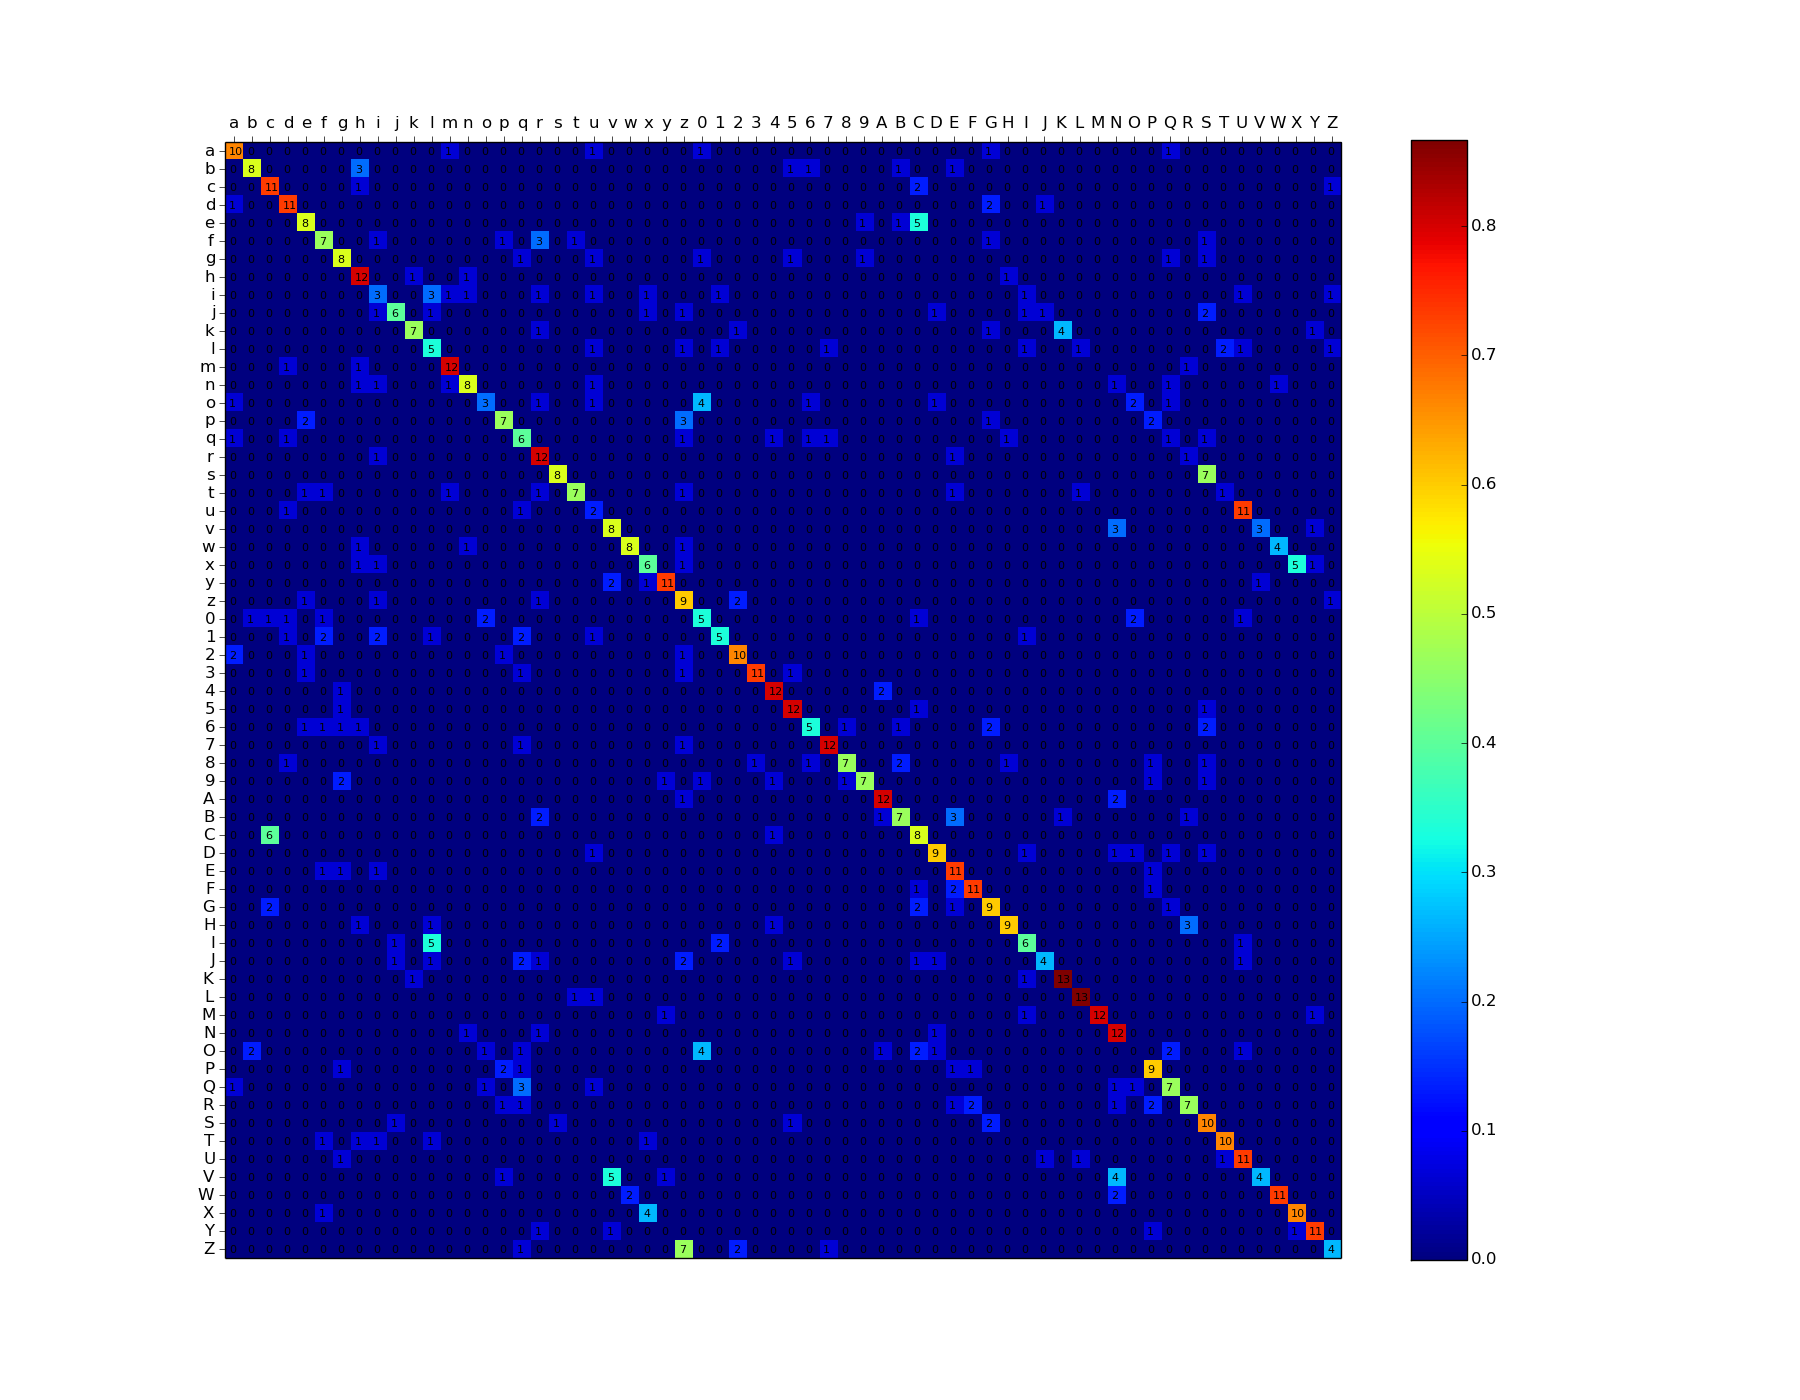
\includegraphics[scale=0.4]{img/resultados/mixtas/best_mean_matrix_Alpha0,01_2040-4.png}}
				\caption[Mixtas Matriz expon]{Matriz de correlación del gráfico \ref{fig: Mixtas-media-mejor} para el mejor resultado.}
				\label{fig: Mixtas-Matrix-media-mejor}
			\end{figure}

			\begin{figure}[!htbp]
				\centerline{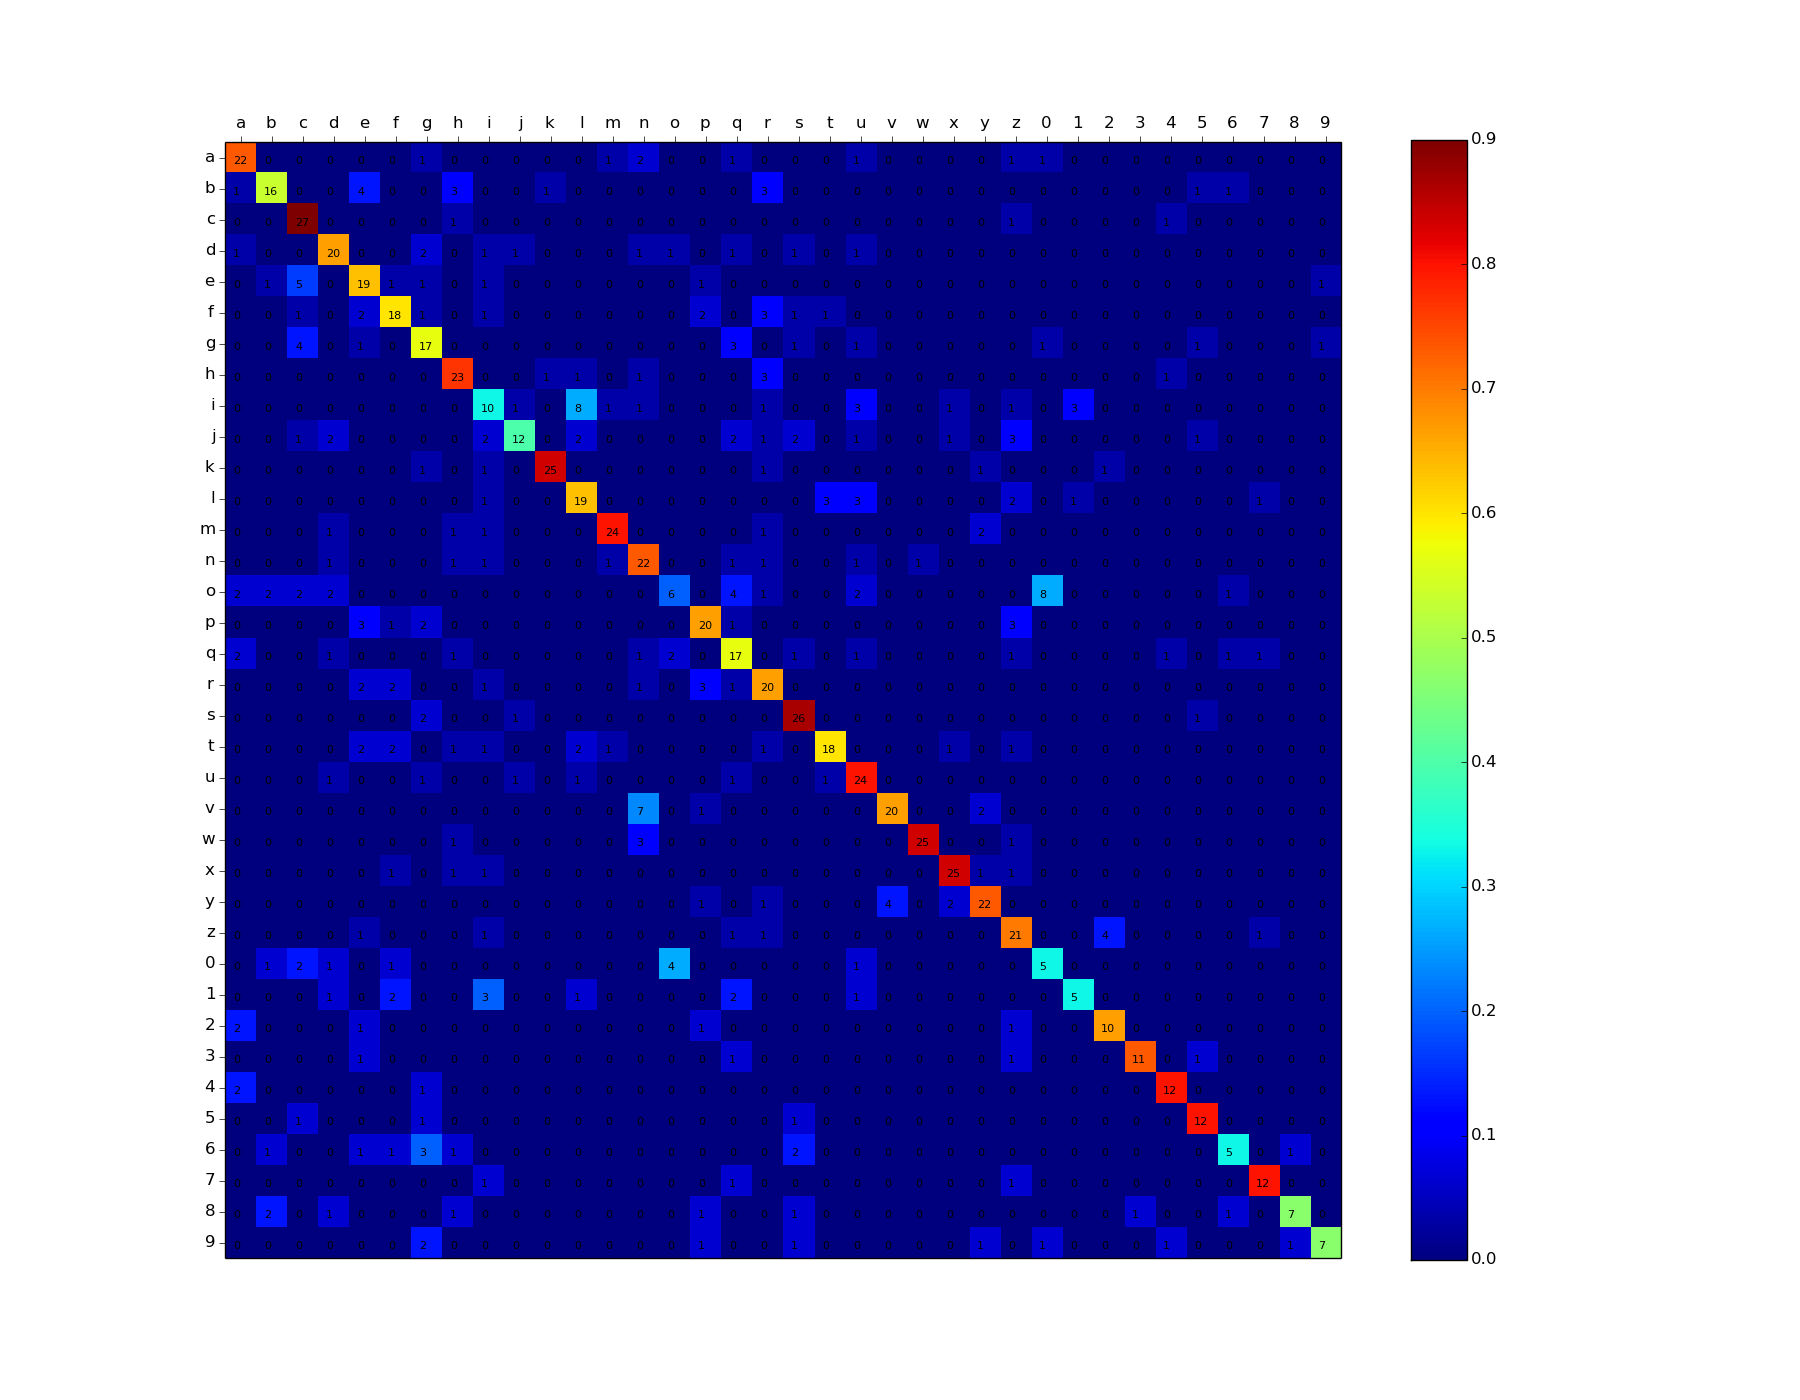
\includegraphics[scale=0.4]{img/resultados/mixtas/best_mean_matrix_Alpha0,01_2040-4_ins.png}}
				\caption[Matriz de correlación ``case insensitive'' para mixtas media]{Matriz de correlación del gráfico \ref{fig: Mixtas-media-mejor} para el mejor resultado no teniendo en cuenta los caracteres en mayúscula.}
				\label{fig: MatrizIns-Mixtas-media-mejor}
			\end{figure}

	
	%\subsection{Conjuntos de Entrenamiento}

	En esta sección se va a discutir los diferentes conjuntos de entrenamientos usados en los experimentos. En las evaluaciones se trabaja básicamente con 3 conjuntos.
	
	El primero, es el compuesto sólo por imágenes de caracteres segmentados de escenas naturales.
	
	El segundo conjunto es el armado con imágenes sintéticas, cuyo proceso de creación fue explicado en detalle en la sección \ref{subsection:impl_propia}. El grupo de imágenes de fuentes que se usa para crear los caracteres sintéticos fue extraído del dataset mencionado anteriormente en \ref{subsection:evaluacion} y consiste en 1000 imágenes por clase. De este conjunto se crearon 6 variaciones diferentes, con el objetivo de observar el impacto que tiene la cantidad de caracteres sintéticos al momento de clasificar imágenes de caracteres naturales. La cantidad de muestras por clase (variaciones) en cada conjunto de entrenamiento es el siguiente:
	\begin{itemize}
		\item Muestras por clase : $ mpc \in \{ 50,100,250,500,1000,2000\}$
	\end{itemize}

	El tercer tipo está compuesto por una combinación de los dos primeros conjuntos. Se creó con la finalidad de observar el impacto en la clasificación de integrar en diferentes proporciones imágenes sintéticas y reales al conjunto de entrenamiento. Dada la escasa cantidad de imágenes naturales para el entrenamiento (15 en total por cada clase) se busca complementar esto integrando datos sintéticos. Por consiguiente se decide crear 9 conjuntos de entrenamiento donde en cada uno se incorporan diferentes proporciones de imágenes sintéticas a las 15 reales que existentes. La proporción de cada conjunto de entrenamiento es de la siguiente manera: 
	
	$$(15, x) x \in \{0,3,8,15,30,75,150,300,750,1500 \}$$
	
	El primer elemento de la tupla $(15, x)$ corresponde a la cantidad de imágenes reales, cuyo valor es fijo. El segundo elemento de la tupla hace referencia a la proporción de caracteres sintéticos. Es fácil observar que a medida que aumentamos la proporción, la cantidad de caracteres naturales se va volviendo cada vez más despreciable. El hecho de no considerar imágenes sintéticas inicialmente $(15,0)$ tiene como finalidad el observar el cambio que se produce desde el inicio cuando no hay caracteres sintéticos en el entrenamiento. Los resultados se analizan en la última sección del presente capítulo.
	
	
	
	%\subsection{Diseño de los experimentos}

	\begin{itemize}
		\item Aca debería ir una descripción de los parámetros a usar en los experimentos con una explicación de lo que se espera obtener.
		\begin{itemize}
			\item Explicar para qué sirve cada parámetro
			\item Explicar los valores que se van a usar para cada parámetro
		\end{itemize}
	\end{itemize}

	Dada la gran cantidad de parámetros que hay en el sistema, la cantidad de experimentos para encontrar la mejor configuración es extensa.

        \paragraph{Generación de datos sintéticos}

	El primer parámetro a considerar es el tipo de conjunto de entrenamiento a evaluar, como se procederá a explicar en la próxima sección, tenemos un total de 20 conjuntos diferentes. Esto con el objetivo de evaluar la performance del clasificador en diferentes ámbitos. Los parámetros utilizados durante la creación de las imágenes sintéticas son, como se explicó en el capítulo anterior, escala, rotación, blur, ruido gaussiano e inclinación. Dado que hay un abanico bastante grande valores para asignarles a estas transformaciones, se decidió por asignarle a cada una un rango de valores los cuales si bien modificaban la imagen, no la hacían ilegible. Dado que los autores en \cite{wang} no especifican el rango de valores para las transformaciones afines que utilizan, se procedió a establecer el siguiente conjunto de rangos para todas las tranformaciones utilizadas:
	
	\begin{itemize}
		\item Inclinación: factor de inclinación $n \in [-0.20 ; 0.20]$
		\item Suavizado gaussiano (blur): $\sigma \in [0 ; 2]$
		\item Escala: es igual en ambos ejes $x=y \in [0.8; 1.25]$
		\item Rotación: en radianes $\theta \in (-0.1; 0.1)$
		\item Ruido gaussiano: $\sigma \in [1; 30]$
	\end{itemize}
	
	El hecho de no contar con una replica exacta del conjunto de datos sintéticos usados por Wang et al., los conjuntos generados con estos valores claramente van a ser distintos a los originales y por ende la comparación de resultados  en \ref{subsection:resultados} va a estar influida por la forma en que se generaron los conjuntos.
	
	\paragraph{Extracción de características con HOG}

	Posteriormente tenemos los parámetros propios que utiliza HOG para extraer las características de cada imagen. HOG hace uso de dos parámetros, la cantidad de \textit{orientaciones} y la cantidad de \textit{celdas por bloque}. Como se explicó en el capítulo anterior \ref{subsection:hog}, dada una imagen, esta se dividía en regiones llamadas celdas. Dentro de cada una se realiza el calculo de las orientaciones y posteriormente dado un bloque de celdas se extraía un histograma de orientaciones de todas las celdas involucradas. Dada la gran cantidad de combinaciones entre ambos parámetros, se decidió por utilizar los siguientes valores:
	
	\begin{itemize}
		\item Orientaciones: $\{8; 9\}$
		\item Celdas por bloque: $\{4; 9\}$
	\end{itemize}
	
	La elección de estos números se debe a que reducen la tasa de errores de clasificación. Un análisis similar se puede encontrar en \cite{DT05} donde los autores (quienes crearon HOG) analizan la mejor configuración para resolver el problema de detección de personas. Si bien el problema que se busca resolver en este trabajo es totalmente diferente, los parámetros que ellos usan para HOG muestran buenos resultados en este problema también.

	\paragraph{Binarización}

	HOG devuelve descriptores de tamaño fijo dependiendo de la cantidad de orientaciones y celdas por bloque que le asignemos. Lo que buscamos con establecer una longitud variable, es evaluar la perdida o ganancia de información sobre la imagen al realizar esto y ver si hay algun impacto en la performance al final. Para poder realizar este ``estiramiento'' o ``reducción'' de los vectores, nos aprovechamos del proceso de binarización explicado anteriormente. El impacto producido al realizar esto es notable y se va a detallar al final del capítulo. Las dimensiones con las que se trabajan es otro parámetro (para los experimentos con imágenes sintéticas y mixtas). Los valores con los que trabajamos son los siguientes:

	\begin{itemize}
		\item Dimensión del vector final: $\{ 240; 480; 1080; 2040;  4080 \}$
	\end{itemize}
	
	La elección de estas dimensiones está directamente relacionada con el siguiente parámetro que es la cantidad de \textit{grupos} por vector, por lo cual estas dimensiones tienen que ser divisibles por cada uno de los grupos a evaluar
	
	Como último parámetro a destacar en la binarización, y lo consideramos como uno de los más importantes, es el método aplicado al momento de generar el umbral de binarización. Como se podrá ver en la subsección de Resultados del capítulo 4, es muy grande el impacto obtenido en la precisión final del clasificador debido a este parámetro. La elección de qué método utilizar fue libre con el objetivo de evaluar cual era el que otorgaba mejores resultados. Se trabajaron con los siguientes métodos:

	\begin{itemize}
		\item Media
		\item Mediana
		\item Bootstrap
		\item Exponencial
	\end{itemize}
	
	Dado que los autores en \cite{wang} no especifican que método usaron al momento de binarizar los vectores. Proponemos estos cuatro métodos. Al igual pasó con los parámetros para generar los datos sintéticos, en el \cite{wang} no se aclara que método se utilizó para la binarización de los vectores, con lo cual todos los resultados obtenidos en los experimentos realizados con imágenes reales y sintéticas van a ser distintos de los originales por más de que, en el caso de las imágenes reales, se usen los mismos conjuntos de entrenamiento y prueba. \RC{Discutir esto, IMPORTANTE.}
		
	\paragraph{Entrenamiento}

	En la etapa de entrenamiento, hay 2 parámetros: la cantidad de bits por \textit{grupo} que determina finalmente la cantidad de grupos en la que se divide cada vector y \textit{alpha} que es un parámetro de inicialización para las tablas. La cantidad de grupos en las que se divide un vector impacta en el tamaño de las tablas y en la clasificación posterior. La cantidad bits denotan la cantidad de dimensiones de cada grupo, por lo cual  la cantidad de grupos esta dado por la división entre la dimensión total del vector y la dimensión del grupo.

	El parámetro \textit{alpha} es necesario ya que las tablas no se pueden inicializar con el valor $0$. Esto es debido ya que, como se explico en la sección \ref{subsection:ferns}, al momento de evaluar una imagen de prueba, puede darse el caso de que se acceda a una posición de la tabla que nunca fue entrenada por lo cual la probabilidad se hace 0 y es un inconveniente para los cálculos posteriores. Los valores por encima de 1 no son convenientes para inicializar las tablas pues afectan a los resultados al momento de normalizarlas.

	\begin{itemize}
		\item Dimensión del grupo: $\{ 1; 2; 4; 8; 10; 12 \}$
		\item Alpha: $\{ 0.01; 0.1; 1 \}$
	\end{itemize}


	%\newpage
\subsection{Resultados}
\label{subsection:resultados}
	tablas, gráficos, análisis y recomendaciones
	\begin{itemize}
		\item Aca debería explicar como fueron procesados los
                  resultados y que tipo de resultados se van a mostrar (ej. los
                  que tuvieron mejor y peor performance). \JS{hay que empezar a
                  poner cuales se van a mostrar y discutir}
                \item \JS{Baseline. Comparar con Wang}
		\item Resultados de dataset con imagenes reales.
		\begin{itemize}
			\item Se presentan los mejores resultados y los parámetros con los cuales se obtuvieron. Se van a presentar los gráficos de los 2 mejores resultados junto con sus matrices de confusión.
			\item Idem pero con los peores resultados obtenidos.
		\end{itemize}
		\item Idem con dataset sintéticos
		\item Idem con dataset sintéticos + reales.

	\end{itemize}
	
	Primero van a ir los resultados de Wang extraidos del paper y expuestos en una tabla. Se tiene que explicar que el resultado obtenido por Wang es el baseline para los experimentos realizados. Un vez que presente los mejores resultados obtenidos vuelvo a generar la tabla de comparacion.
	
	\begin{table}
		\centering
	    \begin{tabular}{ | l | l | l | p{5cm} |}
    			\hline
    				\textbf{Implementación} & \textbf{Score} \\ \hline
    				Wang NATIVE+FERNS & 0.54\% \\ \hline
    				Wang SINT+FERNS & 0.47\% \\
    			\hline
    		\end{tabular}	
    		\caption{Resultados obtenidos por Wang et al. en \cite{wang}}
	\end{table}

	Resultados de haber entrenado y evaluado al clasificador con imagenes reales. Básicamente busco mostrar que llegamos a resultados similares con Wang. Despues de mostrar los resultados, se puede agregar una tabla chiquita comparativa de los resultados.
	
			\begin{figure}[htbp!]
				\centering
				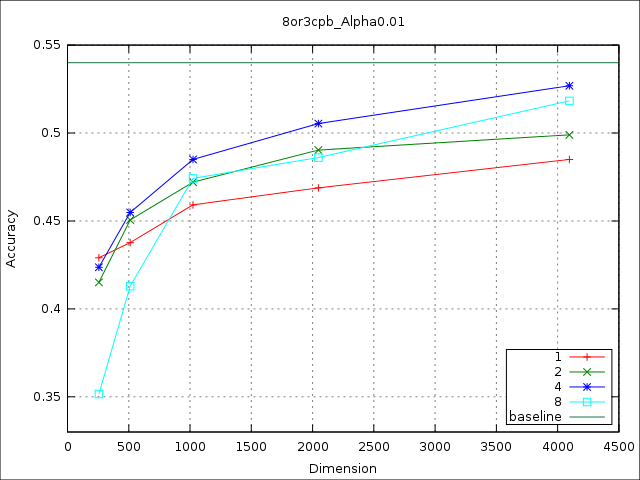
\includegraphics[scale=0.6]{img/resultados/reales/media_8or3cpb_Alpha0,01.png}
				\caption[Reales con umbral media]{Resultado de haber usado la media para el calculo del umbral. La mejor clasificación se logra con los siguientes parámetros: \textit{alpha:0.01}, \textit{bits por grupo: 4}, \textit{dim del vector: 4096}, \textit{orientaciones: 8}, \textit{celdas por bloque: 9}.}
				\label{fig: Reales-media-8or9cpbAlph0.01}
			\end{figure}
			
			\begin{figure}[htbp]
				\centering
				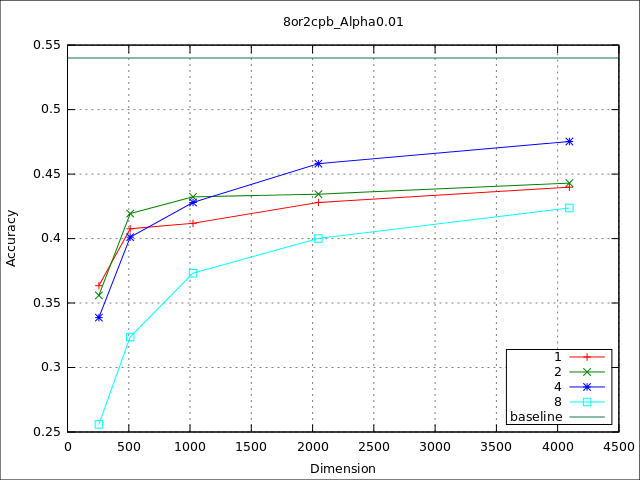
\includegraphics[scale=0.6]{img/resultados/reales/median_8or2cpb_Alpha0,01.png}
				\caption[Reales con umbral mediana]{Resultado de haber usado la mediana para el calculo del umbral. La mejor clasificación se logra con los siguientes parámetros: \textit{alpha:0.01}, \textit{bits por grupo: 4}, \textit{dim del vector: 4096}, \textit{orientaciones: 8}, \textit{celdas por bloque: 4}.}
				\label{fig: Reales-mediana-8or4cpbAlph0.01}
			\end{figure}
			
			\begin{figure}[htbp]
				\centering
				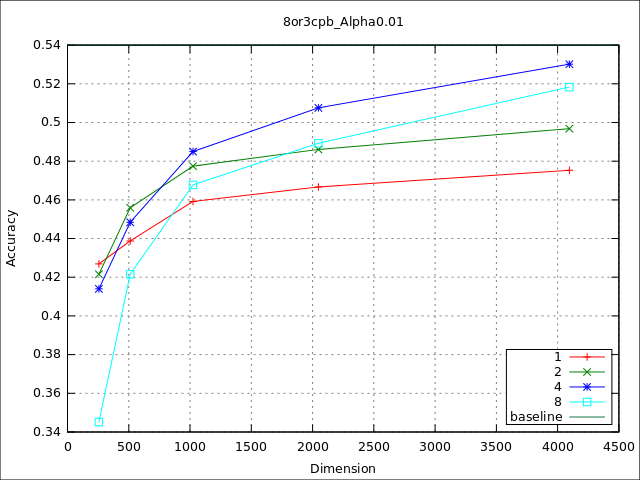
\includegraphics[scale=0.6]{img/resultados/reales/expon_8or3cpb_Alpha0,01.png}
				\caption[Reales con umbral exponencial]{Resultado de haber usado la distribución exponencial para el calculo del umbral. La mejor clasificación se logra con los siguientes parámetros: \textit{alpha:0.01}, \textit{bits por grupo: 4}, \textit{dim del vector: 4096}, \textit{orientaciones: 8}, \textit{celdas por bloque: 9}.}
				\label{fig: Reales-expon-8or9cpbAlph0.01}
			\end{figure}
			
			\begin{figure}[htbp]
				\centering
				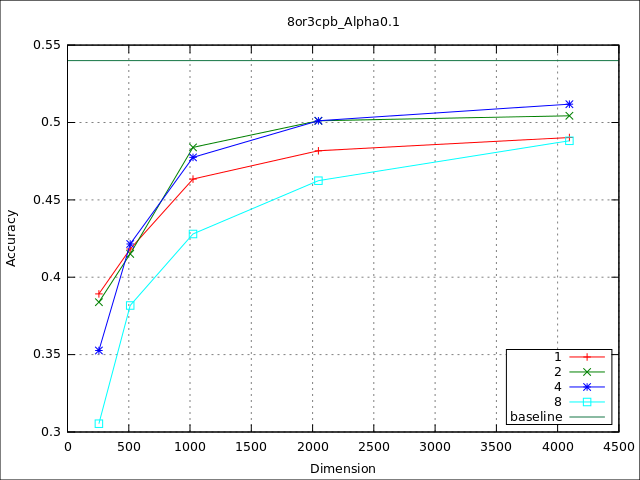
\includegraphics[scale=0.6]{img/resultados/reales/bootstrap_8or3cpb_Alpha0,1.png}
				\caption[Reales con umbral boostrap]{Resultado de haber usado bootstrap para el calculo del umbral. La mejor clasificación se logra con los siguientes parámetros: \textit{alpha:0.1}, \textit{bits por grupo: 4}, \textit{dim del vector: 4096}, \textit{orientaciones: 8}, \textit{celdas por bloque: 9}.}
				\label{fig: Reales-bootstrap-8or9cpbAlph0.1}
			\end{figure}
			
		Después de presentar estos gráficos aclaro que los siguientes experimentos se realizaron utilizando la mejor configuración observada (8 orientaciones, 9 grupos por bloque). Comparación final con los resultados de Wang.
	\begin{table}
		\centering
		\begin{tabular}{ | l | l | l | p{5cm} |}
    			\hline
    				\textbf{NATIVE + FERNS} & \textbf{Score} \\ \hline
    				Wang et al. & 0.54\% \\ \hline
    				Media & 0.53\% \\ \hline
    				Mediana & 0.47\%\\ \hline
    				Exponencial & 0.53\% \\ \hline
    				Bootstrap & 0.51\%\\ 
    			\hline
    		\end{tabular}
    		\caption{Tabla comparativa entre el resultado obtenido por Wang para imágenes naturales y los obtenidos en el presente trabajo, utilizando los cuatro umbrales propuestos.}
    	\end{table}
    	
    	Teniendo en cuenta el resultado de Wang para las imágenes sintéticas, paso a mostrar 
los resultados de haber ido incrementando la proporcion de muestras sintéticas al momento de entrenar al clasificador.

			\begin{figure}[htbp]
				\centering
				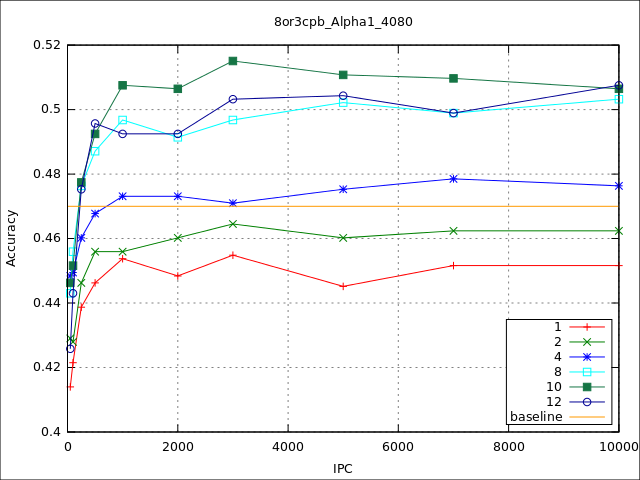
\includegraphics[scale=0.6]{img/resultados/sinteticas/best_media_8or3cpb_Alpha1_4080.png}
				\caption[Sintéticas media bajo resultado]{}
				\label{fig: Sinteticas-media-bajo}
			\end{figure}
			
			\begin{figure}[htbp]
				\centering
				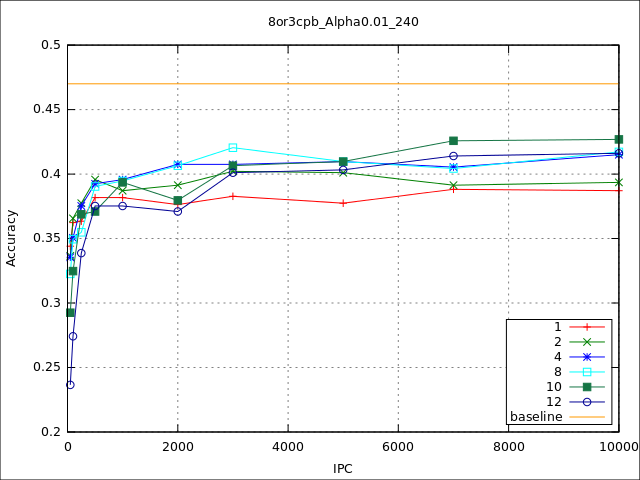
\includegraphics[scale=0.6]{img/resultados/sinteticas/worst_media_8or3cpb_Alpha0,01_240.png}
				\caption[Sintéticas media mejor resultado]{}
				\label{fig: Sinteticas-media-mejor}
			\end{figure}
			
			\begin{figure}[htbp]
				\centering
				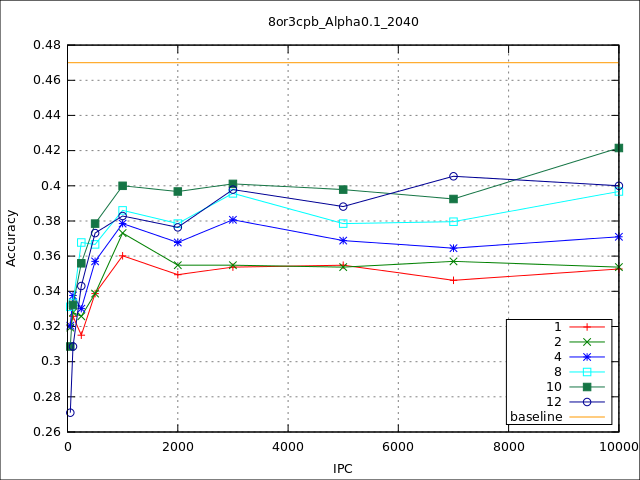
\includegraphics[scale=0.6]{img/resultados/sinteticas/best_median_8or3cpb_Alpha0,1_2040.png}
				\caption[Sintéticas mediana mejor resultado]{}
				\label{fig: Sinteticas-median-mejor}
			\end{figure}
	
			\begin{figure}[htbp]
				\centering
				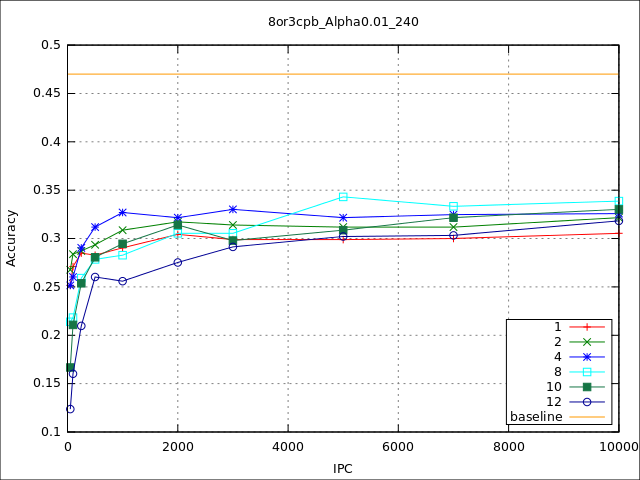
\includegraphics[scale=0.6]{img/resultados/sinteticas/worst_median_8or3cpb_Alpha0,01_240.png}
				\caption[Sintéticas mediana peor resultado]{}
				\label{fig: Sinteticas-median-bajo}
			\end{figure}
				
			\begin{figure}[htbp]
				\centering
				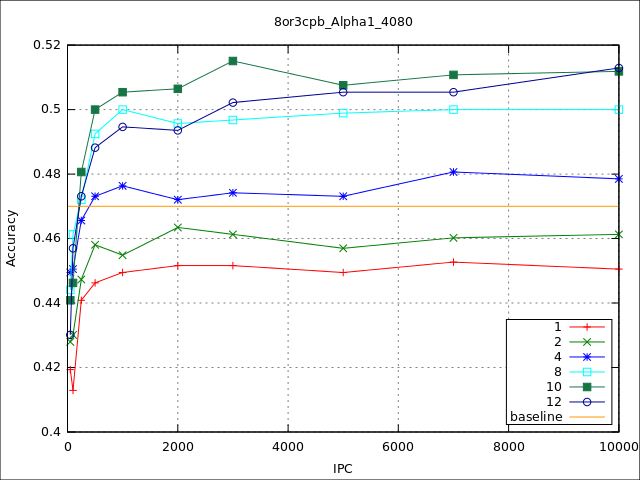
\includegraphics[scale=0.6]{img/resultados/sinteticas/best_expon_8or3cpb_Alpha1_4080.png}
				\caption[Sintéticas exponencial mejor resultado]{}
				\label{fig: Sinteticas-expon-mejor}
			\end{figure}
	
			\begin{figure}[htbp]
				\centering
				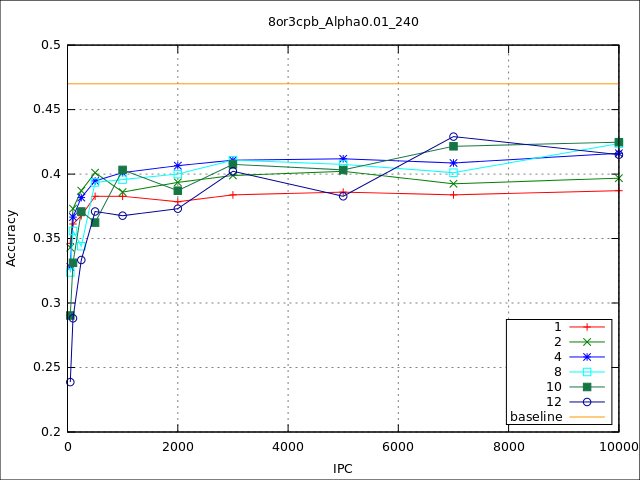
\includegraphics[scale=0.6]{img/resultados/sinteticas/worst_expon_8or3cpb_Alpha0,01_240.png}
				\caption[Sintéticas exponencial peor resultado]{}
				\label{fig: Sinteticas-expon-bajo}
			\end{figure}
			
			\begin{figure}[htbp]
				\centering
				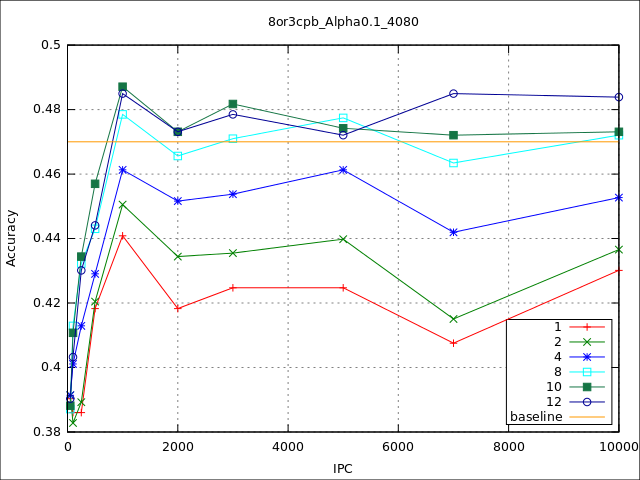
\includegraphics[scale=0.6]{img/resultados/sinteticas/best_bootstrap_8or3cpb_Alpha0,1_4080.png}
				\caption[Sintéticas bootstrap mejor resultado]{}
				\label{fig: Sinteticas-bootstrap-mejor}
			\end{figure}
	
			\begin{figure}[htbp]
				\centering
				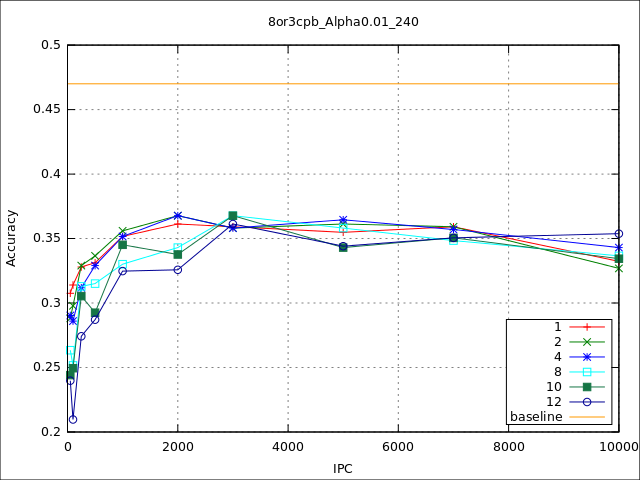
\includegraphics[scale=0.6]{img/resultados/sinteticas/worst_bootstrap_8or3cpb_Alpha0,01_240.png}
				\caption[Sintéticas bootstrap peor resultado]{}
				\label{fig: Sinteticas-bootstrap-bajo}
			\end{figure}

	%\newpage
\subsection{Análisis}
	Análisis / discusión
	\begin{itemize}
		\item Comparar la performance al usar diferentes datasets (comparar cantidad de imágenes por clase al usar caracteres sintéticos). Hacer una tabla.
		\item Observaciones sobre errores de clasificación. El problema que surge con algunos caracteres donde no se puede distinguir minúscula de mayúscula con lo cual se producen errores. Mostrar la matriz de confusión del mejor caso donde no se distingan mayúsculas de minúsculas. Otro error donde ciertos caracteres como la "l" se confunden con otros caracteres como el "1".
		\item Comparar en los resultados con los obtenidos por Wang et al. en condiciones similares. Básicamente explicar algo que no explican en su trabajo Wang et al. y que es la influencia en la cantidad de muestras sintéticas por clase.
		\item Análisis de como aumenta la performance de clasificación el mezclar imágenes sintéticas y reales. Mostrar como a medida que aumentamos demasiado la proporción de img. sintéticas, se tiende a disminuir la precisión. Básicamente, la precisión baja para "igualarse" a la precisión obtenida cuando se entrena al clasif con puras imagenes sintéticas (usando la misma cant. de img. por clase).
	\end{itemize}


	%\subsection{Implementación}

	\begin{itemize}
		\item Explicar porque uso python + las librerías involucradas.
		\item Porque uso JSON y no MySQL para almacenar datos.
		\item Datasets usados y su creación.
		\item Pipeline implementado desde la creación del dataset hasta la obtención de resultados del clasificador Random Ferns.
	\end{itemize}

	

